{\small
\textbf{Bandwidth overheads with a fixed cutoff.}
In \S\ref{sec:eval}, we explained that {\sys} applies a cutoff to the DP
shaped buffer length (if the sampled noise is very large) that depends on the
number of active flows. This reveals the number of active flows at any given
time.
To hide the number of flows, we can set
the cutoff to a fixed~value (\eg based on the
maximum flows that the system must support).

\Cref{subfig:bw-vs-dpInt-video-no-max} presents results similar to those of
\Cref{fig:video-overhead-vs-dpInt}, but with the cutoff for the shaped buffer
length set to a fixed value of 1.21 GB, 1.22 GB, and 1.7 GB.
%(corresponding to 1000 flows).
%for the three DP intervals.
\Cref{subfig:bw-vs-dpInt-web-no-max} presents results similar to those of
\Cref{fig:web-overhead-vs-dpInt} but with cutoffs of 60.8~MB, 60.8~MB, and 110.9
MB.
%
\Cref{subfig:bw-comparison-video-no-max,subfig:bw-comparison-web-no-max} show
the results similar to those of
\Cref{fig:video-overheads-compare,fig:web-overheads-compare}.
%the relative bandwidth overhead of {\ns} compared with {\pacer} and
%{\constshape}.
%In comparison with Pacer, for a small number of parallel flows, {\sys}'s
%bandwidth overhead increases significantly. However, with multiple concurrent
%flows, the amortization effect exponentially reduces overhead.
%
The fixed cutoffs correspond to 1000 flows, which lead to a significant increase
in {\sys}'s overheads.
However, the overheads quickly amortize with several concurrent flows.
}
%\Cref{subfig:bw-vs-dpInt-video-no-max} shows the relative bandwidth overhead of
%our video streaming application for different DP intervals with the shaped
%buffer length cutoff set to 1000 flows.
%Compared to \Cref{fig:video-overhead-vs-dpInt}, {\sys}'s bandwidth overhead
%increases significantly with a fixed cutoff.
%However, the overheads quickly amortize with larger number of concurrent flows.
%%when operating with just a single client, often reaching two orders of
%%magnitude higher values.
%%However, the overheads remain relatively the same when a large number of
%%clients are present (e.g., 128 or more).
%\Cref{subfig:bw-vs-dpInt-web-no-max} represents the similar results for the web
%service.

\begin{figure}[t]
    \centering
    \begin{subfigure}{0.49\columnwidth}
        \centering
        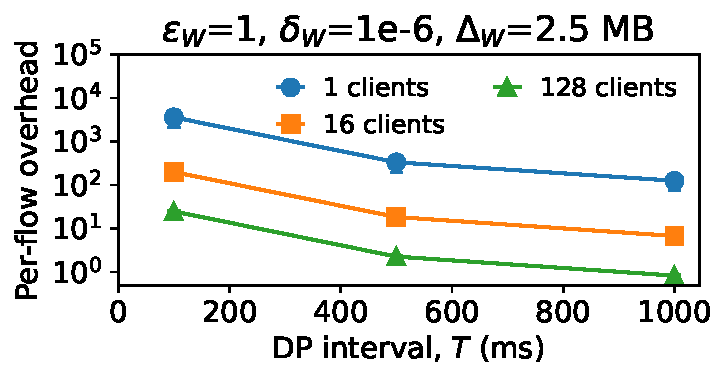
\includegraphics[width=\textwidth]{overhead_vs_dp_interval_video_updated_no_max.pdf}
        \caption{Video streaming}
        %        \caption{Noise vs privacy loss}
        \label{subfig:bw-vs-dpInt-video-no-max}
    \end{subfigure}
    \hfill
    %    \begin{subfigure}{0.33\textwidth}
        %        \centering
        %
        %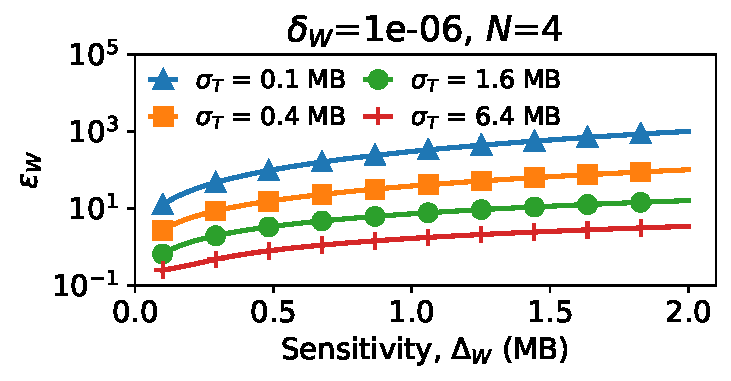
\includegraphics[width=\textwidth]{plots/privacy_loss_VS_sensitivity_video.pdf}
        %        \caption{Sensitivity vs privacy loss}
        %        \label{subfig:high-sensitivity-epsilon-sensitivity}
        %    \end{subfigure}
    %    \hfill
    \begin{subfigure}{0.49\columnwidth}
        \centering
        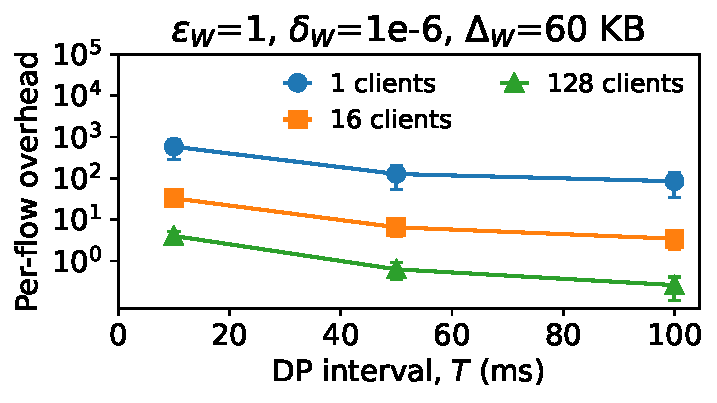
\includegraphics[width=\textwidth]{overhead_vs_dp_interval_web_updated_no_max.pdf}
        \caption{Web service}
        %        \caption{\# of DP queries vs privacy loss}
        \label{subfig:bw-vs-dpInt-web-no-max}
    \end{subfigure}
    %  \caption{
        %    \update{Bandwidth overheads with a fixed cutoff.}
        %%    \am{Make notations consistent.}
        %  }
    %\end{figure}


    %\begin{figure}[t]
    \centering
    \begin{subfigure}{0.49\columnwidth}
        \centering
        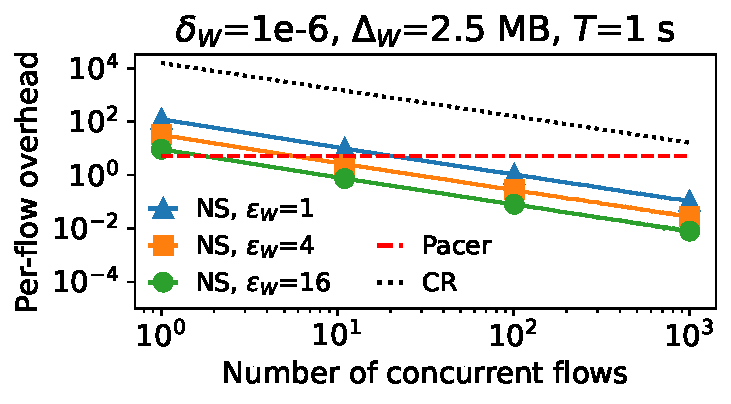
\includegraphics[width=\textwidth]{overhead_vs_number_of_traces_video_bidirectional_loglog_updated_no_max.pdf}
        \caption{Video streaming}
        %        \caption{Noise vs privacy loss}
        \label{subfig:bw-comparison-video-no-max}
    \end{subfigure}
    \hfill
    %    \begin{subfigure}{0.33\textwidth}
        %        \centering
        %
        %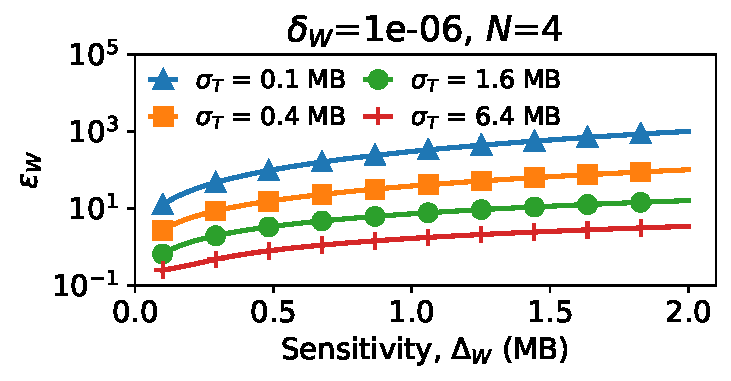
\includegraphics[width=\textwidth]{plots/privacy_loss_VS_sensitivity_video.pdf}
        %        \caption{Sensitivity vs privacy loss}
        %        \label{subfig:high-sensitivity-epsilon-sensitivity}
        %    \end{subfigure}
    %    \hfill
    \begin{subfigure}{0.49\columnwidth}
        \centering
        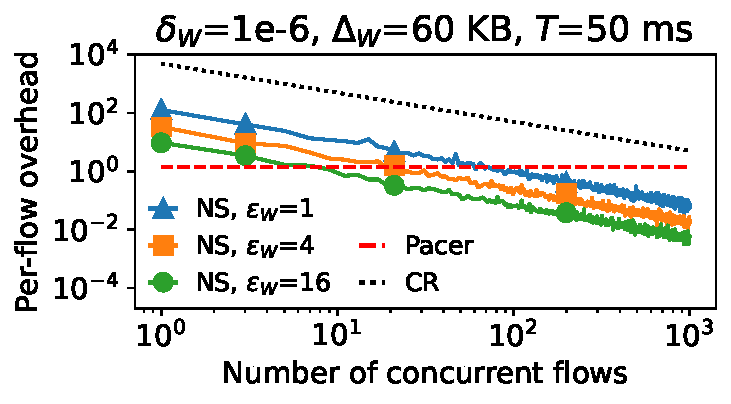
\includegraphics[width=\textwidth]{overhead_vs_number_of_traces_web_bidirectional_loglog_updated_no_max.pdf}
        \caption{Web service}
        %        \caption{\# of DP queries vs privacy loss}
        \label{subfig:bw-comparison-web-no-max}
    \end{subfigure}
    \caption{
        \update{Bandwidth overheads with a fixed cutoff.}
        %    \am{Make notations consistent.}
    }
\vspace{-0.4cm}
    %  \caption{
        %    \update{Comparison of {\sys}, constant shaping, Pacer with a fixed
        %cutoff.}
        %%    \am{Make notations consistent.}
        %  }
\end{figure}

